% This is a sample document using the University of Minnesota, Morris, Computer Science
% Senior Seminar modification of the ACM sig-alternate style. Much of this content is taken
% directly from the ACM sample document illustrating the use of the sig-alternate class. Certain
% parts that we never use have been removed to simplify the example, and a few additional
% components have been added.

% See https://github.com/UMM-CSci/Senior_seminar_templates for more info and to make
% suggestions and corrections.

\documentclass{sig-alternate}
\usepackage{color}
\usepackage{graphicx}
\usepackage{mathtools}
%\usepackage[colorinlistoftodos]{todonotes}

%%%%% Uncomment the following line and comment out the previous one
%%%%% to remove all comments
%%%%%\newcommand{\comment}[1]{}
\newcommand{\comment}[1]{{\bf \tt  {#1}}}
%%%%% NOTE: comments still occupy a line even if invisible;
%%%%% Don't write them as a separate paragraph
\newcommand{\todo}[1]{\textcolor{magenta}{\comment{Todo: {#1}}}}

\begin{document}

% --- Author Metadata here ---
%%% REMEMBER TO CHANGE THE SEMESTER AND YEAR
\conferenceinfo{UMM CSci Senior Seminar Conference, May 2015}{Morris, MN}

\title{Monte Carlo Tree Search and Its Applications}

\numberofauthors{1}

\author{
% The command \alignauthor (no curly braces needed) should
% precede each author name, affiliation/snail-mail address and
% e-mail address. Additionally, tag each line of
% affiliation/address with \affaddr, and tag the
% e-mail address with \email.
\alignauthor
Max Magnuson\\
	\affaddr{Division of Science and Mathematics}\\
	\affaddr{University of Minnesota, Morris}\\
	\affaddr{Morris, Minnesota, USA 56267}\\
	\email{magnu401@morris.umn.edu}
}

\maketitle
\begin{abstract}

\end{abstract}

\keywords{Monte Carlo Tree Search, Heuristics, Upper Confidence Bounds, Artificial Intelligence}

\section{Introduction} 
In 1997 the field of artificial intelligence(AI) experienced a monumental breakthrough when IBM's Deep Blue defeated Garry Kasparov, a reigning grand master, in a chess match\cite{TheGrandChallenge}. The researchers were able to achieve this by using brute force deterministic tree searching methods combined with human knowledge of chess. The human knowledge allows the AI to evaluate the strategic value of a move much like a grand master would, and then populate a tree to search for the best move. This event demonstrated to the world the power of computers and artificial intelligence. 

While computers are capable of outplaying the top players of chess, they struggle when it comes to board games like Go\cite{TheGrandChallenge}. Go is a board game about positional board advantage which is something traditional AI struggles with. They struggle because moves in Go tend to have very long dependencies. A single move may have major effects on moves 50 to 100 moves ahead\cite{RAVEinGo}. This makes game trees for Go significantly deeper than chess. Go also has many more moves available to the player at any time than chess. This makes the game trees for Go much wider than in chess. These problems cause deterministic approaches to perform poorly. It is just too much for those approaches to efficiently handle.

People have started turning to alternative methods to approach Go. One such method, Monte Carlo tree search(MCTS), has had a lot of success in Go. MCTS eschews the typical brute force tree searching methods, and it utilizes statistical processes and heuristic approaches to decide what move to make. In 2009, for the first time ever, a computer defeated a top professional Go player in a 9x9 game\cite{TheGrandChallenge}. It took twelve years for AI to advance from defeating Garry Kasparov to achieve its first major victory in Go, and it was only on the smallest board that Go is played on.

MCTS has been growing in popularity in recent years, and it demonstrates a lot of promise. In this paper we will be examining MCTS and a few of its applications.  
\section{Background}
MCTS combines the random sampling of traditional Monte Carlo methods with tree searching. Monte Carlo methods use repeated random sampling to obtain results. The random sampling is used to construct a game tree. This tree will be traversed based on statistical processes, and the MCTS method relies on the convergence of the traversal to reliably choose the best move. The traversal is in convergence when the traversal selects the same path on each traversal. MCTS is a heuristic method and as such it will not always find the optimal move, but it has a reasonably high success of choosing moves that will lead to greater chances of winning.
\subsection{The Tree Structure}\label{sec:TreeStructure}
MCTS structures the game state and its potential moves in a tree. Each node in the tree represents the state of the game with the root node representing the current state. Each line represents a legal move that can be made from one game state to another. In other words, it represents the transformation from the parent node to the child node. Any node may have as many children as there are legal moves. For example, at the start of a game of Tic-Tac-Toe the root node may have up to nine children, one for each possible move. Each following child can only have one less child than its parent since the previous moves are no longer available as options.

\begin{figure}[h]
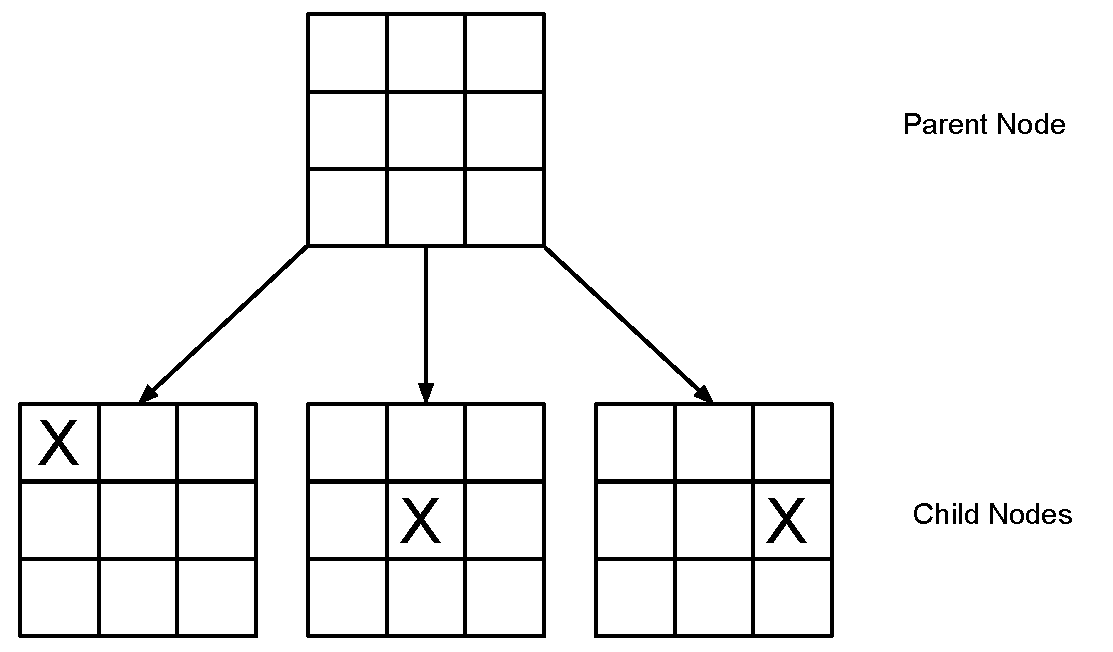
\includegraphics[width=8cm]{TicTacToeTree.pdf}
\centering
\caption{A small portion of what a tree for TicTacToe represents}
\label{fig:TicTacToe}
\end{figure}

Figure \ref{fig:TicTacToe} represents the top portion of a tree for the game Tic-Tac-Toe. The AI is making the first move, so the source node is the first game board. Each child node represents the potential moves that can be made from the current game state. It is important to note here that those are only three of the potential nine child nodes. In the naive implementation of MCTS, each potential child node must be added to the tree before any of those child nodes can be traversed. Other variations of the MCTS algorithm have ways of avoiding this requirement\cite{ActionSelection}. Once MCTS has decided which move to make, the source node of the tree will then become the child it chose. For example, if MCTS chose the left child in figure \ref{fig:TicTacToe}, then the new root node would be that child and every other child node would be discarded. 

Along with the game state, each node contains a value that gives an estimate of wins compared to total games in that subtree. The higher the value, the greater proportion of wins in that subtree. The lower the value, the smaller the proportion of wins in that subtree. By choosing the node with the greatest estimated value, the MCTS algorithm is choosing the path with the most number of wins. This means that the MCTS algorithm is maximizing the number of winning moves it can select. This is what MCTS relies on to be effective.

\subsection{The Four Steps of MCTS}
The process of MCTS is split up into four steps: Selection, Expansion, Simulation, and Backpropagation. These four steps are iteratively applied until a decision from the AI must be made. Typically, there is a set amount of time that the AI has to make its move, so that is when the algorithm will make its decision.

\begin{figure}[h]
	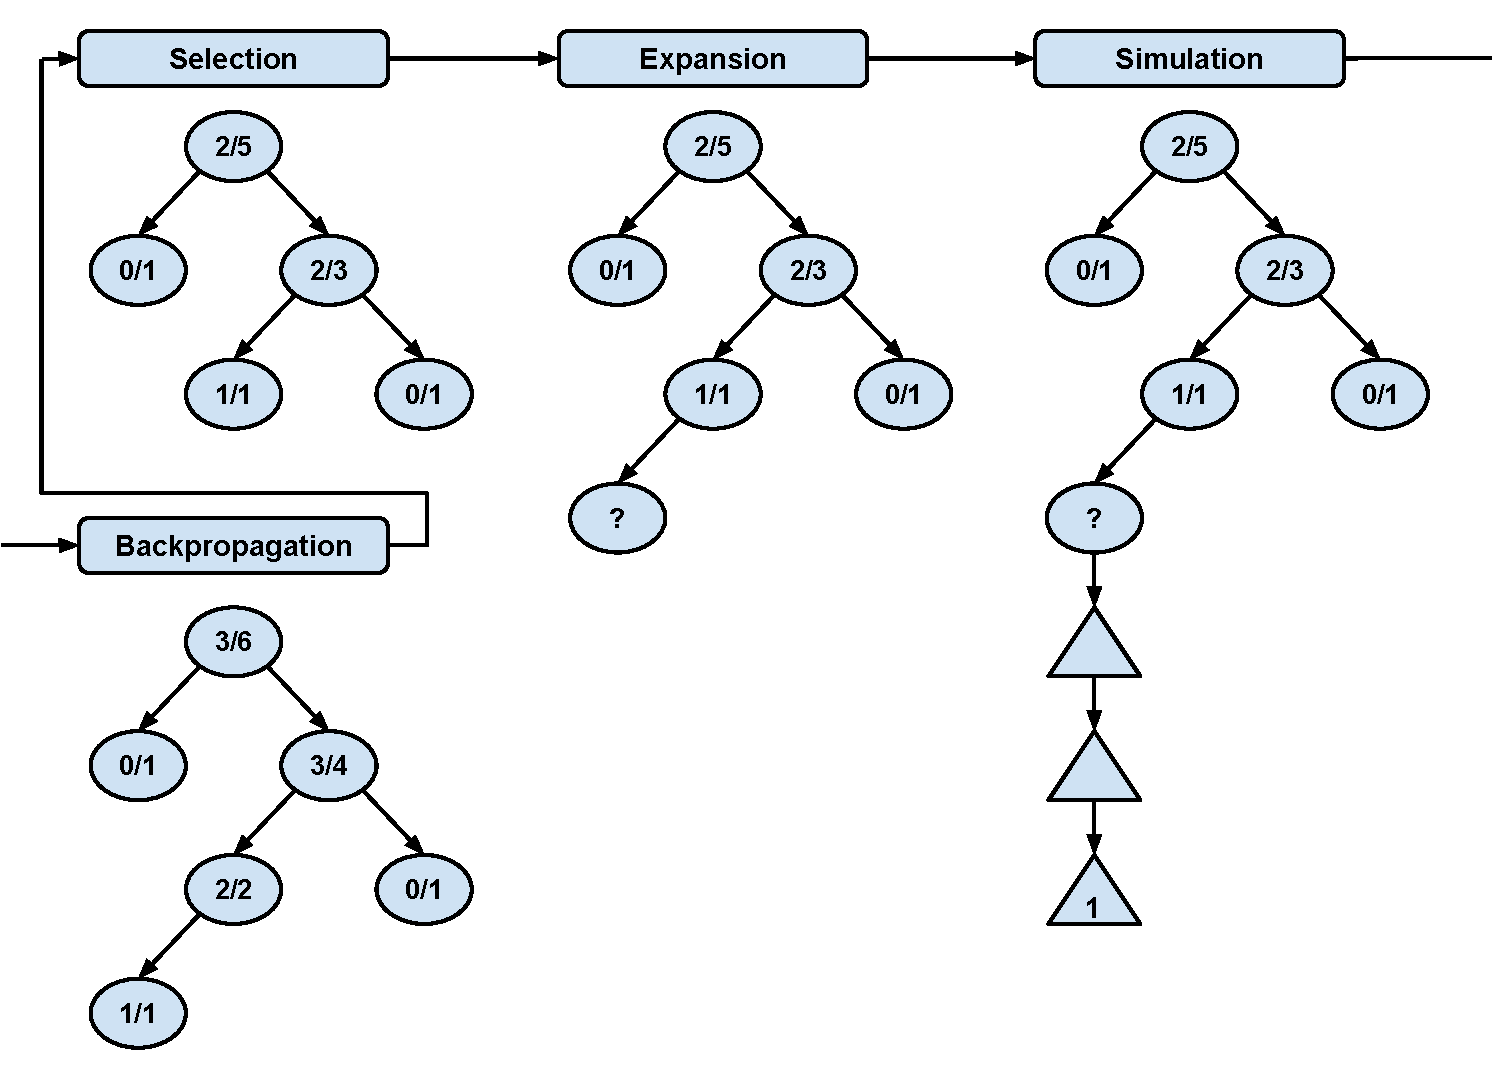
\includegraphics[width=8.5cm]{MCTSFourStepProcess.pdf}
	\centering
	\caption{The four steps of MCTS}
	\label{fig:FourSteps}
\end{figure}

In figure \ref{fig:FourSteps} the first number in each node represents the number of wins in that subtree. The second number is the total number of simulations performed in that subtree which is also the same number of nodes in the subtree. The ratio of these two numbers provide us with the estimated value of each node.

\textbf{Selection} - In the selection process, the MCTS algorithm traverses the current tree using a tree policy. A tree policy uses an evaluation function that prioritize nodes with the greatest estimated value. In figure \ref{fig:FourSteps}, starting from the root node, the tree policy must make a decision between the 0/1 node and the 2/3 node. Since 2/3 is greater than 0/1, the tree policy will choose the 2/3 node in its traversal. Once at the 2/3 node, the tree policy will then choose the 1/1 node because it is greater than 0/1. So now the algorithm is at the 1/1 node as it transitions into the expansion step.

\textbf{Expansion} - In the expansion step, a new node is added to the tree as a child of the node reached in the selection step. The algorithm is currently at the 1/1 node, so there is a child node added onto that node indicated by the node with the ?. There is only one node added to the tree in each iteration, and it is at this step.

\textbf{Simulation} - In this step, a simulation(also referred to as a playout or rollout) is performed by choosing moves until either an end state or a predefined threshold is reached. In the case of Go or TicTacToe, an end state is reached when the game ends. Then based on the result of the simulation, the value of the newly added node is established. For example, a simulation for a node in Go reaches the end of a game(the end state), and then determines a value based on whether the player won or lost. In figure \ref{fig:FourSteps} the simulation ended in a 1. Therefore, the value of the new node is 1/1. One simulation resulted in a win, and one simulation has been performed.

In the simulation process, moves are played out according to the simulation policy\cite{ActionSelection}. This policy may be either weak or strong. A weak policy uses little to no predetermined strategy. It chooses moves randomly from either a subset of the legal moves or from all of the legal moves. A policy may prefer a certain subsection of moves because those moves might be more favorable. Perhaps in the game of TicTacToe the corners are considered to be more favorable. We incorporate this into a simulation policy by having the algorithm randomly choose corner moves until there are no more corner moves left. Then the policy will choose moves at random from the rest of the legal moves. A strong policy uses a more guided approach to choosing moves. A strong policy may make the simulation too deterministic or make it more prone to error\cite{TheGrandChallenge}, so a weak policy is generally preferred. 

\textbf{Backpropagation} - Now that the value of the newly added node has been determined, the rest of the tree must be updated. Starting at the new node, the algorithm traverses back to the root node. During the traversal the number of simulations stored in each node is incremented, and if the new node's simulation resulted in a win then the number of wins is also incremented. In figure \ref{fig:FourSteps} only the nodes with values 0/1 are not updated since they are not a parent of the newly added node. This step is very important because it ensures that the values of each node accurately reflect simulations performed in the subtrees that they represent.

\subsection{Upper Confidence Bound}

The upper confidence bound applied to trees(UCT) is used by MCTS as the tree policy in the selection step to traverse the tree. UCT balances the idea of exploration versus exploitation. The exploration approach promotes exploring unexplored areas of the tree. This means that exploration will expand the tree's breadth more than its depth. While this approach is useful to ensure that MCTS is not overlooking any potentially better paths, it can become very inefficient very quickly in games with a large number of moves. To help avoid that, it is balanced out with the exploitation approach. Exploitation will tend to stick to one path that has the greatest estimated value. This approach is greedy and will extend the tree's depth more than its breadth. UCT balances exploration and exploitation by giving relatively unexplored nodes an exploration bonus.  

 \begin{equation}
 \label{UCTequation}
 UCT(node) = \frac{W(node)}{N(node)} + \sqrt[C]{\frac{ln(N(parentNode))}{N(node)}}
 \end{equation}

When traversing the tree, the child node that returns the greatest value from equation \ref{UCTequation} will be selected~\cite{ActionSelection}. N represents the total number of simulations performed at that node and its descendants. W represents how many of those simulations resulted in a winning state. C represents an exploration constant that is found experimentally. The first part of the UCT takes into consideration the estimated value of the node from the ratio of simulations won to total simulations. This is the exploitation part of the equation. The second part of the UCT is the exploration bonus. This compares the total number of simulations performed at the parent node and its descendants to the total number of simulations performed at the examined node and its descendants. This means that the lower the number of simulations that have been performed at this node, the greater this part of the equation will be. 

\section{Using MCTS to play Go}

MCTS has been very successful in its applications in Go. The computer Go programs MoGo and Crazy Stone both use MCTS, and they have had the best performance of any computer Go programs\cite{RAVEinGo}. Those programs use the naive MCTS algorithm with the UCT approach, and they apply their own variations that take advantage of certain aspects of Go.

\subsection{All Moves as First(AMAF)}
All moves as first(AMAF) is a methodology that treats all moves as if they were the next move played. AMAF does not grant any move extra strategic value based on when it is played. Therefore, in AMAF moves have no contextual dependencies on other moves. This is particularly useful when a move played elsewhere on the board has little or no impact on the move being examined, or if a game arrives at the same state regardless of the order in which the moves are played. 

\begin{figure}[h]
	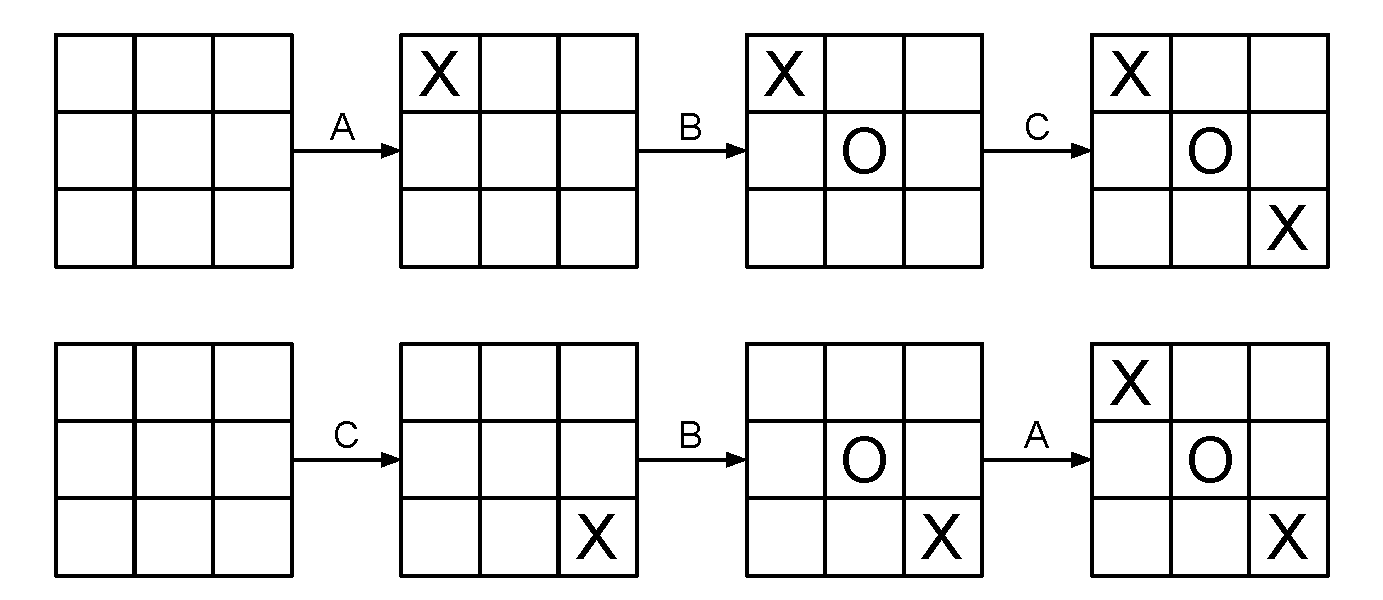
\includegraphics[width=8cm]{MoveOrderNotMattering.pdf}
	\centering
	\caption{Comparison of two sequences of moves in TicTacToe}
	\label{fig:TwoSeq}
\end{figure}

In figure \ref{fig:TwoSeq} are two possible sequences of moves that can be played out in the game TicTacToe. Even though the order of moves A and C are different, it still results in the same game state. AMAF is useful in analyzing the effectiveness of this situation since the order in which the moves are played has no effect strategically. Thus, we can treat playing move A first or move C first as having the same strategic value.

The AMAF methodology is applicable to Go because many of the situations only affect what is happening locally. If a move is made elsewhere on the board, it does not have much of an affect on the strategic value of the move being examined. It is also important to note that in Go a move that repeats a board state is illegal. Therefore, this methodology will not have any inconsistencies with replaying the same move.

\subsection{Rapid Action Value Estimate}
Rapid action value estimate(RAVE) takes the concept of AMAF and applies it to a tree structure. RAVE can be thought of as assigning values to the edges of the tree which represent moves. The value of these moves come from any simulation performed within the subtree in which that move was played. The value is a ratio of these simulations that resulted in a win to the total number of simulations. This is different from MCTS in that MCTS chooses nodes for the strategic value of the game state represented by that node. RAVE chooses nodes for the strategic value of the move.

\begin{figure}[h]
	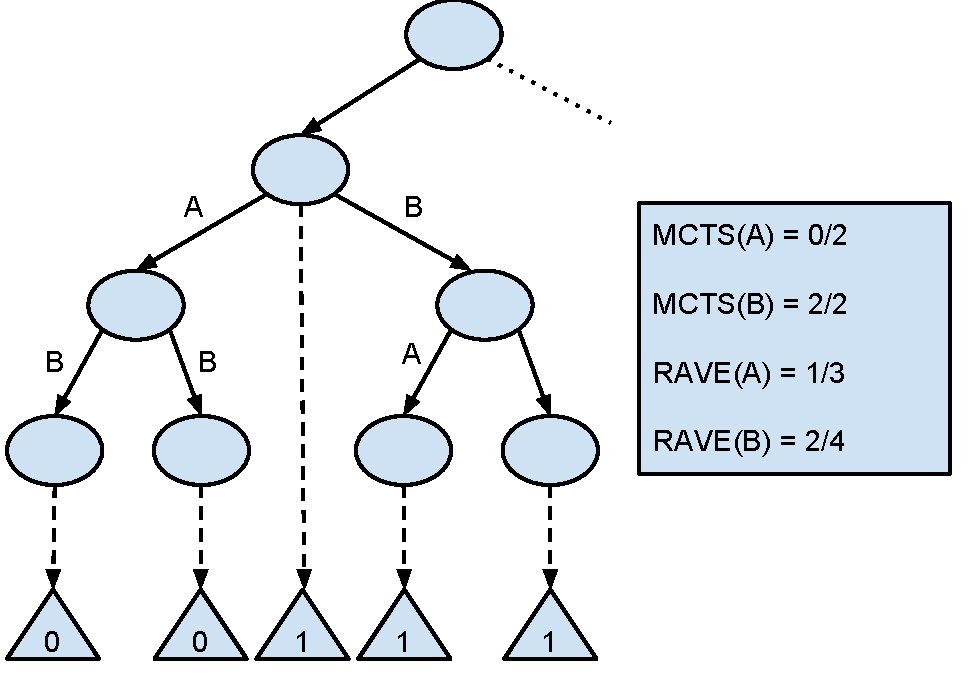
\includegraphics[width=8cm]{RAVEDiagram.pdf}
	\centering
	\caption{MCTS vs RAVE}
	\label{fig:RAVEDiagram}
\end{figure}

Figure \ref{fig:RAVEDiagram} is a comparison between moves A and B from node Z. The triangles represent the result of the simulations performed at each node. In MCTS, the value of A is the value of the node A points to. In this case, A has the value 1/3. Likewise, B has the value 2/3. These values come from the three simulations performed in their respective subtrees. In the RAVE approach, the value for move A is determined by any simulation performed by the descendants of node Z in which A was performed. This accounts for the simulation performed in the subtree of B that used move A. Now in RAVE, the value of A is 2/4. The same is true for the RAVE value of B. B was performed in two other simulations in Z's subtree. This makes the RAVE value of B 2/5.

When determining which node to traverse to from node Z, MCTS and RAVE would produce different results. MCTS would choose the node that B is pointing to because the MCTS value of B is greater than the MCTS value of A. RAVE would choose the node A is pointing to because the RAVE value of A is greater than the RAVE value of B.   

The RAVE approach is very powerful and allows us to retrieve much more information out of every simulation. MCTS only gains one piece of information from each simulation. That information is only the result of the simulation. In RAVE, every move performed in a simulation provides us with information. The strategic value of a move in RAVE is developed much more quickly as a result. This means that trees generated by RAVE converge more quickly than trees generated by MCTS.

\subsection{MC RAVE}
The RAVE approach is very useful and efficient, but it can sometimes select an incorrect move\cite{RAVEinGo}. In Go, when the players have close tactical battles, the sequencing of the moves become very important. In this situation, we cannot treat the moves as AMAF. We still need the contextual dependencies of the MCTS approach.

MC RAVE combines the naive MCTS algorithm and the RAVE approach into one algorithm. MC RAVE stores the values of each node from MCTS and the value of each move from RAVE in the tree structure. MC RAVE takes a weighted average of the two values to determine which node to choose in traversal~\cite{RAVEinGo}. When few simulations have been performed, the RAVE values are given more weight. In this case, RAVE is more accurate because the contextual dependencies of moves are less clear. When a lot of simulations have been performed, the MCTS values will be weighted more heavily. The MCTS values are given more weight because the contextual dependencies of the moves are more strongly developed and are more accurate overall.
\subsection{Results}
AI that use more traditional approaches to playing games have had very little success playing Go. The deterministic approaches struggle to defeat even low rank amateurs. Now with new Go programs implementing MCTS with RAVE, they have achieved a lot of success and the achievements are only growing in number. The top computer programs can now compete with top professionals in 9x9 Go\cite{RAVEinGo}. Not only that, but those programs can even compete against the top pros in handicap games of 19x19 Go. Handicap games let one player start with some number of pieces on the board. That is an incredible feat taking into consideration the immense complexity of a 19x19 board. Clearly, MCTS has demonstrated its impact on AI approaches to Go.

\section{Using MCTS for Narrative Generation}
Automated narrative generation is an interesting problem with many applications. One such application is in video games. Narrative generation provides the user with a unique experience on each playthrough which can extend the amount of enjoyment a user can receive from a single game. Another application for narrative generation is as a learning tool. Generating an endless number of fun and interesting stories provides plenty of material for reading practice. These are only two examples, but there are many more.

Kartal et al\cite{Narrative} decided to apply MCTS to narrative generation. MCTS is a promising approach to narrative generation because as with Go it shares the same problem of expansive search spaces. With each additional character, item, location, or action, the number of possible narratives grows exponentially. Given the success in Go, with its huge search spaces, it makes sense to apply MCTS to narrative generation.

\subsection{Description of Narratives}

The researchers' algorithm uses various predefined actors(or characters), items, locations, and actions to generate a narrative. Actions are used to have actors, items, and locations interact with one another. Here are a few possible actions:
\begin{itemize}
\item \textbf{Move(A, P):} A moves to place P.
\item \textbf{Kill(A, B):} B's health to zero(dead).
\item \textbf{Earthquake(P):} An earthquake strikes at place P. This causes people at P to die (health=0), items to be stuck, and place P to collapse.
\end{itemize}
Each action has a name and in the parentheses are the actors, items, or places used by the action. The action move for example takes a character A and moves them to place P. Actions are important because they are what progress the story. 

In the researchers algorithm, the user does not provide any of the actions used by the algorithm. However, the user defines the initial setup and goals for the narrative. An initial setup indicates where actors or items are located. The inspector is in his office, or the lamp is at Becky's house. The narrative goals are what the user wishes to occur in the story. Perhaps the user would like there to be at least two murders and for the murderer to be captured. Given this information, the algorithm will attempt to generate a believable narrative that satisfies the goals set by the user.

\subsection{Tree Representation}
As stated in section \ref{sec:TreeStructure}, the nodes of the MCTS tree represent the entire state at that node. In narrative generation, it is a little different. Each node only represents a specific step(or action) of the story instead of capturing the entirety of the narrative up to that point. In order to retrieve the current narrative up to that node, we would need to traverse up the tree all the way to the root node. This structuring is similar to the MCTS tree for Go in that to know the sequence of moves leading up to a node, we would need to traverse back to the root. A node by itself does not provide us with the order in which moves are played, only the current state of the game.

In addition to encoding for an action, each node also keeps track of various attributes. Attributes are characteristics of an actor that help keep track of the current state of the story. An attribute of an actor might be that actors current health. The health of an actor may go down if attacked. Another example of an attribute is the location of an actor. It would not make much sense if an actor traveled to a location that they are already at which would be possible if the location of the character is not stored.

\subsection{Evaluation Function}\label{sec:EvalFunction}
MCTS requires a method of evaluating a simulation and the value of a node. In Go or other games, the result of a simulation is if it ended in a win or a loss. The value of a node is then the ratio of simulations won to total simulations. This method of evaluation does not apply to narrative generation. There is no winning or losing. Therefore, the researchers needed to develop their own metric for evaluating the narratives generated by the MCTS algorithm.

The researchers decided that a function which considers both the believability of the story and the number of goals it completes, would be appropriate for evaluating a narrative~\cite{Narrative}. Both believability and goal completion must be considered because it does not make for a quality narrative without either. A narrative could easily complete the goals defined by the user without being very believable, and a narrative could be very believable while not accomplishing any of the goals. Sometimes this results in one being sacrificed for the other. Maybe a long series of actions, that are not the most believable, are used for the sake of completing the goals of the narrative. While this outcome is not perfect, it is preferable over the two extremes.

The believability of a narrative is determined from the product of the believability of all of the actions performed. The believability of a certain action is determined based on its context within the current state of the narrative. This means that certain actions are more or less believable based on previous events or attributes. Character A killing character B is less believable if character A is not angry at character B. Character A looking for clues at character B's house is more believable given that character A is a detective. Each action has its own user defined scale of believability ranging from 0 to 1~\cite{Narrative}, and the result from this scale is what is factored into the overall believability. Since the overall believability is a product of each action's believability, the overall believability ranges from 0 to 1 as well.

Believability is not the only important metric for narrative generation. It is also important that a story completes most, if not all, of the goals defined by the user. The researchers addressed this by determining the percentage of the goals the narrative completes. This percentage is then combined with the believability of the story by taking their product. Now, the evaluation function considers both the believability and goal completion of a story. 

\subsection{Search Heuristics}
\todo{Put this somewhere}
The method for tree generation in the authors' application of MCTS is very similar to the naive MCTS. The main difference is in the simulation step. For the simulation step, the researchers implemented a threshold to determine when the simulation should end. The simulation will end when either the narrative has reached a certain length, or if the narrative accomplishes a sufficient percentage of goals. This is different than in Go because the end state is not always the end of a narrative. Once the end of the simulation is reached, the simulation will be evaluated using the evaluation function outlined in section \ref{sec:EvalFunction}.

The researchers implemented two different search heuristics into their MCTS variation. One heuristic uses selection biasing during the traversal of the tree, and the other uses a rollout biasing while performing simulations.

The selection biasing approach uses a table to store the average value, as determined by the evaluation function, of a certain action. During the traversal of the tree, the algorithm will use this value in combination with the value of a node to determine which node to traverse to next. The traversal uses a weighted average between the two values. The value from the table is weighted more heavily with fewer simulations, and the value of the node is weighted more heavily with more simulations. This approach is much like the RAVE approach used in Go, but the values are stored in a table instead of in the tree. As such the value from the table is the average value of that action anytime it has been used in any part of the tree. This is different from the RAVE approach in that, RAVE only takes the value of the move within a subtree.

The other heuristic the researchers implemented is called rollout biasing. This biasing is applied during the simulation step in MCTS. The rollout biasing uses a table, just like the selection biasing, to keep track of the average value of an action. This value is used to bias the random selection during the simulation process. If the average value of an action in the table is fairly high, then it is more likely for that action to be chosen. Likewise, if the average value of an action from the table is fairly low, then the action is less likely to be chosen. It is important to make clear that the process is still random. This means that due to random chance, there will still be variety in the narratives generated by each simulation.
 
\subsection{Tree Pruning}
The trees generated by MCTS can get very memory intensive, so the authors implemented tree pruning into their algorithm to allow for the algorithm to use the memory it is allocated more efficiently. In tree pruning, an algorithm will selectively cut out pieces of the tree that do not seem very promising. This process allows the algorithm to reallocate that memory for future nodes. 

The authors only allow their MCTS algorithm to plan out the narrative one step at a time. When selecting for the next step, the algorithm runs for a predefined number of iterations. After those iterations are performed, the algorithm chooses the node with the greatest potential value from the child nodes of the previously chosen action. The chosen node effectively becomes the new root node of the tree while keeping track of the steps that preceded it. When the new node is chosen, all other children from the previous node are discarded. The memory that those nodes were allocated can now be used for future simulations. This process allows for the algorithm to much more efficiently use the memory it is allocated.

The authors do make note that this approach makes the algorithm no longer probabilistically complete. This means that it is possible that one of the pruned branches could be preferable to the current path. The current path may just be a local maxima instead of the preferred global optimum. The global optimum in this case is considered the best possible narrative. Even with this flaw, the authors still found their algorithm to perform reasonably well.

\subsection{Results}
The authors compared their implementation of the MCTS algorithm to three different deterministic tree search algorithms: Breadth-First Search, Depth-First Search, and Best-First Search\cite{Narrative}. Each of these algorithms should provide the optimal solution if given enough time and memory. Depth-First Search and Best-First search in particular have the opportunity of finding the solution very early on in the search.

These four algorithms were compared given a low budget of 100 thousand nodes and a high budget of three million nodes. The predefined user goal was to have at least two actors killed, and for the murderer to be arrested. Each of the algorithms were run a total of three times for each budget. Each of the three narratives returned were evaluated and averaged with scores ranging from 0 to 1. Then the resulting values were compared. 

When given a low budget, the only algorithm that came close to MCTS, was the Breadth-First Search algorithm. Bread-First Search scored a value of 0.05, while MCTS scored a 0.07. The other two algorithms scored below 0.01. When given the high budget of three million nodes, MCTS far and away outperformed the other algorithms. MCTS scored 0.9 while the others did not even reach 0.01~\cite{Narrative}.

The authors found that the Depth-First search failed to meet any of the goals of the narrative. The Best-First search attempted to complete the user defined goals while only using believable actions, but it used up its allocated memory in trying to do so. Breadth-First search performed the best of the three deterministic algorithms, but its actions tended to not be very believable in accomplishing goals.

The authors also compared their two different search heuristics. One algorithm used the selection biasing heuristic. The second algorithm used the rollout biasing heuristic, and the third algorithm used neither. The three were compared using the same conditions as before. Given a low budget, the MCTS algorithm with selection biasing outperformed the other two algorithms. Given a high budget, the selection biasing algorithm found a local minima and could not outperform the MCTS algorithm without either biasing. The rollout biasing algorithm did show quite the improvement over the traditional MCTS algorithm by doubling its value to 0.45.

Additionally, the authors compared their tree pruning approach to a MCTS algorithm without it. The two algorithms were run on the same machine and were allowed run until they ran out of memory. The MCTS algorithm without tree pruning usually failed when exploring around five million nodes. The MCTS  algorithm with tree pruning could search over 50 million nodes without running out of memory. Not only did this approach require much less memory, but it would find a narrative with a much higher value.

\section{Conclusions}

\section{Acknowledgements}

% The following two commands are all you need in the
% initial runs of your .tex file to
% produce the bibliography for the citations in your paper.
\bibliographystyle{abbrv}
% sample_paper.bib is the name of the BibTex file containing the
% bibliography entries. Note that you *don't* include the .bib ending here.
\bibliography{MaxMagnusonSeniorSeminar}  
% You must have a proper ".bib" file
%  and remember to run:
% latex bibtex latex latex
% to resolve all references

\end{document}
